% Vehicle Detection Diagram
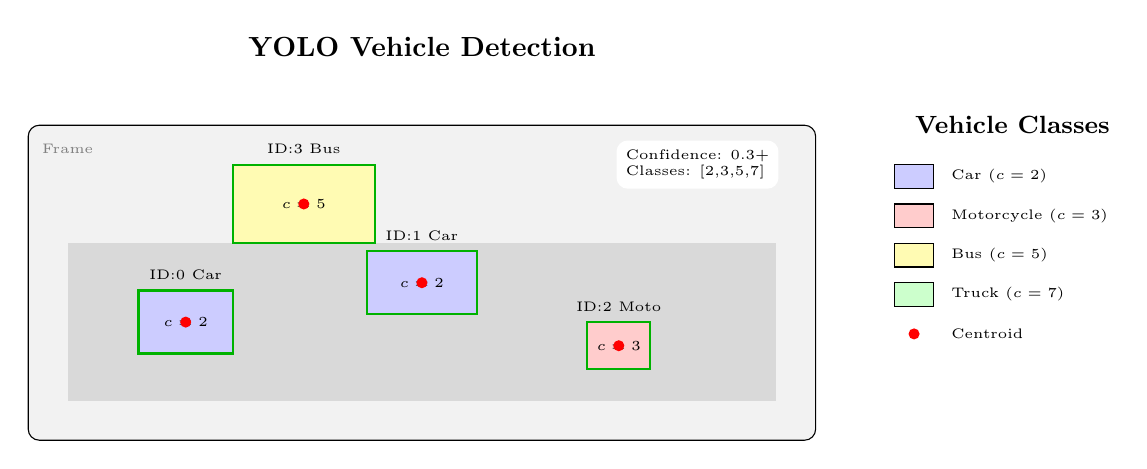
\begin{tikzpicture}[
    box/.style={
        rectangle,
        draw=green!70!black,
        thick,
        minimum width=1.2cm,
        minimum height=0.8cm
    }
]

% Title
\node[font=\bfseries] at (5, 5) {YOLO Vehicle Detection};

% Frame background
\draw[fill=gray!10, rounded corners] (0, 0) rectangle (10, 4);
\node[font=\tiny, gray] at (0.5, 3.7) {Frame};

% Road area
\fill[gray!30] (0.5, 0.5) -- (9.5, 0.5) -- (9.5, 2.5) -- (0.5, 2.5) -- cycle;

% Vehicles (bounding boxes)
\node[box, fill=blue!20, label={[font=\tiny]above:ID:0 Car}] (v0) at (2, 1.5) {};
\node[font=\tiny] at (2, 1.5) {$c=2$};

\node[box, fill=blue!20, minimum width=1.4cm, label={[font=\tiny]above:ID:1 Car}] (v1) at (5, 2) {};
\node[font=\tiny] at (5, 2) {$c=2$};

\node[box, fill=red!20, minimum width=0.8cm, minimum height=0.6cm, label={[font=\tiny]above:ID:2 Moto}] (v2) at (7.5, 1.2) {};
\node[font=\tiny] at (7.5, 1.2) {$c=3$};

\node[box, fill=yellow!30, minimum width=1.8cm, minimum height=1cm, label={[font=\tiny]above:ID:3 Bus}] (v3) at (3.5, 3) {};
\node[font=\tiny] at (3.5, 3) {$c=5$};

% Centroids
\fill[red] (2, 1.5) circle (2pt);
\fill[red] (5, 2) circle (2pt);
\fill[red] (7.5, 1.2) circle (2pt);
\fill[red] (3.5, 3) circle (2pt);

% Legend
\node[font=\small\bfseries] at (12.5, 4) {Vehicle Classes};
\draw[fill=blue!20] (11, 3.2) rectangle (11.5, 3.5);
\node[font=\tiny, right] at (11.6, 3.35) {Car ($c=2$)};
\draw[fill=red!20] (11, 2.7) rectangle (11.5, 3);
\node[font=\tiny, right] at (11.6, 2.85) {Motorcycle ($c=3$)};
\draw[fill=yellow!30] (11, 2.2) rectangle (11.5, 2.5);
\node[font=\tiny, right] at (11.6, 2.35) {Bus ($c=5$)};
\draw[fill=green!20] (11, 1.7) rectangle (11.5, 2);
\node[font=\tiny, right] at (11.6, 1.85) {Truck ($c=7$)};

\fill[red] (11.25, 1.35) circle (2pt);
\node[font=\tiny, right] at (11.6, 1.35) {Centroid};

% Detection info
\node[font=\tiny, align=left, fill=white, rounded corners] at (8.5, 3.5) {
    Confidence: 0.3+\\
    Classes: [2,3,5,7]
};

\end{tikzpicture}




